\documentclass[tikz,border=2pt]{standalone}
\usepackage{amsmath,amssymb}
\usepackage{tikz}
\usepackage{pgfplots}
\pgfplotsset{compat=1.18}

\begin{document}
% Bananas: Weibull demand with shape k = 2 and scale lambda = 50, beta = 13/15; the shaded
% probability 13/15 ends at y* = 50 sqrt(-ln(2/15)) = 70.97 kg.
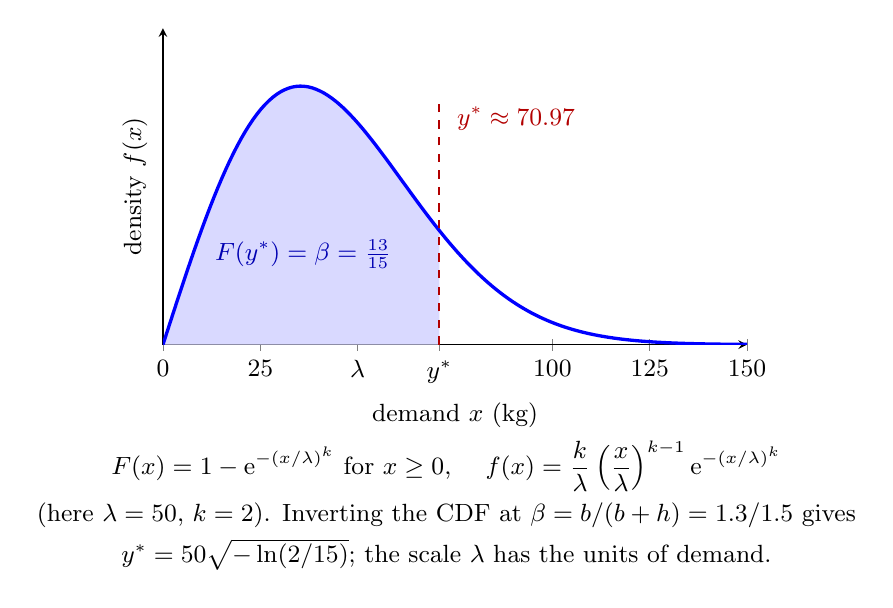
\begin{tikzpicture}
	\begin{axis}[width=9cm, height=5.6cm, xlabel={demand $x$ (kg)}, ylabel={density $f(x)$}, xmin=0, xmax=150, ymin=0, ymax=0.021, axis lines=left, tick label style={font=\small}, label style={font=\small}, xtick={0,25,50,70.97,100,125,150}, xticklabels={0,25,$\lambda$,$y^*$,100,125,150}, ytick=\empty, samples=150]
		\addplot[fill=blue!15, draw=none, domain=0:70.97] {(2/50)*(x/50)*exp(-(x/50)^2)} \closedcycle;
		\addplot[blue, very thick, domain=0:150] {(2/50)*(x/50)*exp(-(x/50)^2)};
		\draw[red!70!black, dashed, thick] (axis cs:70.97,0) -- (axis cs:70.97,0.016);
		\node[font=\small, blue!70!black] at (axis cs:36,0.006) {$F(y^*)=\beta=\tfrac{13}{15}$};
		\node[anchor=west, font=\small, red!70!black] at (axis cs:73,0.015) {$y^*\approx70.97$};
	\end{axis}
	\node[anchor=north, align=center, font=\small] at (3.6,-1.1) {$F(x)=1-\mathrm{e}^{-(x/\lambda)^k}$ for $x\ge0$, \quad $f(x)=\dfrac{k}{\lambda}\left(\dfrac{x}{\lambda}\right)^{k-1}\mathrm{e}^{-(x/\lambda)^k}$\\[3pt] (here $\lambda=50$, $k=2$). Inverting the CDF at $\beta=b/(b+h)=1.3/1.5$ gives\\[4pt] $y^*=50\sqrt{-\ln(2/15)}$; the scale $\lambda$ has the units of demand.};
\end{tikzpicture}
\end{document}
